\chapter{CNN Conecepts}

\section{Lesson Outline}
\href{https://www.youtube.com/watch?v=zS4iCL3lDtU&ab_channel=Udacity}{Youtube} \newline

In this lesson we are going to learn the general concepts underlying Convolutional Neural Networks (CNNs), and how they relate to the neural networks you already know, Multi-layer Perceptrons (MLPs).\newline

We will start by applying MLPs to the images of a very famous computer vision dataset, then see the limitations of MLPs when it comes to images.\newline

We'll then learn how Convolutional Neural Networks solve these limitations, allowing them to outperform MLPs for all image tasks.\newline

Finally, we will introduce at a high level the conceptual underpinnings of CNNs that make them so powerful and useful.

\section{MNIST Dataset}
\href{https://www.youtube.com/watch?v=a7bvIGZpcnk&t=1s&ab_channel=Udacity}{Youtube} 

\subsection{Image Classification and the MNIST Dataset}

Classifying an image means assigning one label to the entire image. The label could be for example the most prominent object in the image ("cat," "dog,"...), or a characteristic of the image ("cloudy sky," "sunny sky,"...).

The MNIST database is arguably the most famous dataset in the field of deep learning. It contains 70,000 handwritten digits 0-9 in white over a black background, and the task is to classify each image by assigning it the label corresponding to the depicted number.

It is nowadays considered a solved problem, with modern neural networks having performances that are on par or better than human performances and over 99.9\% accurate. However, it is still widely used for tutorials and in the literature as the first, most obvious benchmark for new ideas.

\section{How Computers Interpret Images}
\href{https://www.youtube.com/watch?v=mEPfoM68Fx4&t=2s&ab_channel=Udacity}{Youtube} \newline

\subsection{Definitions}

Before continuing, let's define some of the terms that we are going to use:

\begin{itemize}
    \item \textbf{Vector} - an array of numbers with only one dimension
    \item \textbf{Matrix} - an array of numbers with two dimensions
    \item \textbf{Array} or tensor - two interchangeable generic terms which can mean arrays with one, two, or n dimensions
\end{itemize}

\subsection{Computer Interpretation of Images}

An image is seen by the computer as an array of values (a matrix). A grid of values for each grid cell is called a pixel, and each pixel has a numerical value.

\includegraphics[width=0.5\linewidth]{img//cnn/image.png}

The images in the MNIST dataset are 28 x 28 and 8-bit grayscale. This means that the computer represents each one of them as a square matrix of 28 x 28 elements, where the value in the element of the matrix represents the light intensity with a range of 0 to 255: 0 means pure black and 255 means pure white.

\includegraphics[width=0.1\linewidth]{img//cnn/image2.png}


\subsection{Normalizing Image Inputs}

Data normalization is an important pre-processing step for neural networks. The activation functions that are normally used in neural networks (sigmoid, ReLU, etc.,...) have the highest rate of change around 0:

\includegraphics[width=1\linewidth]{img//cnn/image3.png}

This means that their derivative is large for inputs that are not too far from 0. Since we train neural networks with gradient descent, the training can proceed faster if the weights stay in the vicinity of where the activation function changes rapidly, i.e., close to 0. \newline

The weights of a neural network are typically initialized with a mean of 0, i.e., some weights are negative and some are positive, but they are in general between -1 and +1, close to 0. Remember that these weights are multiplied with the feature values (in this case the pixel values) and then a bias is added on top before the result is fed to the activation function. \newline

Therefore, if we want the input of the activation function to be somewhere close to 0, we need to start with a number that is close to zero, because two numbers close to zero multiplied together give another number close to zero. \newline

So we need to take the pixels in the input image, which in the case of a grayscale image have values between 0 and 255, and renormalize them to be close to zero. \newline

The easiest way is to just divide the value by 255, thereby changing the pixel values to be between 0 and 1.

\includegraphics[width=1\linewidth]{img//cnn/image-normalized.png}

In many cases, we go further than that: we compute the mean and the standard deviation of all the pixels in the renormalized dataset, then we subtract the mean and divide by the standard deviation for each image separately. Therefore, our transformed data will contain both negative and positive pixels with mean 0 and standard deviation 1. Sometimes you'll see an approximation here, where we use a mean and standard deviation of 0.5 to center the pixel values. If you'd like, you can \href{https://pytorch.org/docs/stable/}{\textbf{read more here about the Normalize transformation in PyTorch.}}


\subsection{Classification with Neural Networks}

We already know how to perform classification with neural networks, and in particular with a Multi-Layer Perceptron (MLP). This network takes as input a grayscale image (a matrix) and outputs a vector of scores or a vector of probabilities (one for each class). The class corresponding to the maximum of that vector corresponds to the best guess for the label of the image.

\subsection{Flattening}

Suppose we want to use an MLP to classify our image. The problem is, the network takes a 1d array as input, while we have images that are 28x28 matrices. The obvious solution is to \textit{flatten} the matrix, i.e., to stack all the rows of the matrix in one long 1d vector, as in the image below.

\includegraphics[width=0.75\linewidth]{img//cnn/flattening-bw.jpeg}
\captionof{figure}{To flatten an image we take the rows and stack them together in a 1d array}
\label{img:flattening}

Using the example of \autoref{img:flattening} with a 4x4 image, we have a matrix with 16 pixel values. Instead of representing this as a 4x4 matrix, we can construct a vector with 16 entries where the first 4 entries of our vector correspond to the first row of our old array,The second 4 entries correspond to the second row, and so on. After converting our images into vectors. they can then be fed into the input layer of an MLP. 

\section{MLP Structure and Class Scores}

\subsection{MLP for Images}
\href{https://www.youtube.com/watch?v=4zFq5U1IHgU&ab_channel=Udacity}{Youtube} \newline


\subsection{A Multi-Layer Perceptron for MNIST}
The input of our MLP must obviously be 28 x 28=784, which corresponds to the dimension of the flattened image. The output of the MLP must also be obviously a vector with 10 elements (one for each class). The values in this vector are proportional to the probability that the network assigns to each class. So if the network thinks that it is most likely that the given image is an 8, then the element in the array corresponding with 8 should be the largest. The output values are also called class scores. Class scores indicate how sure the network is that a given input is of a specific class. The class scores are often represented as a vector of values or even as a bar graph, indicating the relative strengths of the scores. \newline

But what goes between the input and the output? How many hidden layers, and how many neurons?

\includegraphics[width=0.75\linewidth]{img//cnn/mlp.jpeg}
\captionof{figure}{Schematic of a Possible MLP for the Classification of Images in the MNIST Dataset}


\section{Loss and Optimization}
\href{https://www.youtube.com/watch?v=583E6aKwQig&ab_channel=Udacity}{Youtube} \newline

\begin{itemize}
    \item Loss: Measure any mistakes between a predicted and true class
    \item Backpropagation: We can compute the gradient of the loss with respect to the models weights. This way quantify how bad a particular weight is in making a mistake
    \item Optimization: we can choose an optimization function like gradient descent to give us a way to calculate a better weight value.
\end{itemize}

\includegraphics[width=1\linewidth]{img//cnn/image5.png}

We need to make the output layer more interpretable. We apply a \textbf{softmax} activation function to convert these scores into probabilities. \newline

As a model trains, its goal will be to find the weights that minimize this loss function,and therefore it gives us the most accurate predictions. A \textbf{loss function and backpropagation} give us a way to quantify how bad a particular network weight is based on how close a predicted and a true class label are from one another. \newline

Next, we need a way to calculate a better weight value. Think of the loss function as a surface that resembles a mountain range. Then to minimize this function, we need only find a way to descend to the lowest valley. This is the role of an optimizer, the standard method for minimizing the loss and optimizing for the best weight values is called gradient descent. \newline

\subsection{Loss Function}

The \textbf{loss function} quantifies how far we are from the ideal state where the network does not make any mistakes and has perfect confidence in its answers.

Depending on the task and other considerations we might pick different loss functions. For image classification the most typical loss function is the \textbf{Categorical Cross-Entropy (CCE) loss}, defined as: \[CCE = -\sum_{i=1}^{n_{classes}} y_i \log \hat{p}_i\]
where:

\begin{itemize}
    \item The sum is taken over the classes (10 in our case)
    \item yi is the ground truth, i.e., a \href{https://en.wikipedia.org/wiki/One-hot\#Machine_learning_and_statistics}{\textbf{one-hot encoded vector}} of length 10
    \item pi is the probability predicted by the network
\end{itemize}

\begin{quote}
NOTE: In PyTorch it is customary to have the network output class scores (or \textit{logits}) instead of probabilities like in other frameworks. Then, the PyTorch loss function itself will first normalize the scores with a Softmax function, and then compute the CCE loss.

\end{quote}

\includegraphics[width=0.5\linewidth]{img//cnn/image4.png}

\subsection{Gradient Descent}

The values of the weights and the biases in the MLP are optimized by using Gradient Descent (or more precisely Stochastic Gradient Descent or SGD for short), or similar algorithms such as \href{https://optimization.cbe.cornell.edu/index.php?title=Adam}{\textbf{Adam}}. SGD takes the derivative of the loss with respect to the weights and then updates the values of the weights so as to decrease the loss as quickly as possible.

\section{Loading Data and Transforming Images in PyTorch}

\subsection{Loading Images in PyTorch}

\subsubsection{Transforms}

Before we can feed images to a neural network, there are some operations we must perform. As we have seen before, we need to normalize the images so the values in the pixels are floating point numbers between 0 and 1, or -1 and 1, instead of values from 0 to 255 as in the RGB format. We also need to transform them to PyTorch Tensors, so our network can handle them. \newline

In many cases we also want to augment our dataset by performing random transformations, but more on this in a later lesson. \newline

For the moment, let's see how to normalize the images and transform them to tensors:
\begin{lstlisting}
import torchvision.transforms as T

## T.Compose creates a pipeline where the provided
## transformations are run in sequence
transforms = T.Compose(
    [

        # This transforms takes a np.array or a PIL image of integers
        # in the range 0-255 and transforms it to a float tensor in the
        # range 0.0 - 1.0
        T.ToTensor(),

        # This then renormalizes the tensor to be between -1.0 and 1.0,
        # which is a better range for modern activation functions like
        # Relu
        T.Normalize((0.5), (0.5)),
    ]
)
\end{lstlisting}
In many real-world datasets we also need some other operations like resizing, which we will see later.

\subsubsection{Datasets}

PyTorch offers dataset and dataloaders specific for images and their annotations.\newline

A \verb|Dataset| instance provides methods to load and manipulate the data, whereas a \verb|DataLoader| instance wraps the dataset and allows iterations over it during training, validation, and test. \newline

It is possible to define custom datasets when needed, but the \verb|torchvision| library offers specific classes inheriting from the base \verb|Dataset| class for all major computer vision datasets. You can find a list of these datasets \href{https://pytorch.org/vision/stable/datasets.html\#image-classification}{\textbf{here}}. For example, you can load the MNIST dataset just by doing:
\begin{lstlisting}
train_data = datasets.MNIST(
    root="data", train=True, download=True, transform=transforms
)

test_data = datasets.MNIST(
    root="data", train=False, download=True, transform=transforms
)
\end{lstlisting}
\verb|torchvision| also offers an \verb|ImageFolder| class that can be used to extract images and labels directly from a local directory.

You have to structure your data in the following way:

\includegraphics[width=0.5\linewidth]{img//cnn/imagefolder.jpeg}

We need a top-level directory with the name of your dataset (\verb|custom_data| in this case). Then, we need one or more subdirectories representing the classes. In this case we have a dataset of cats and dogs, and accordingly we have two subdirectories with the same name. Within each subdirectory we place the images belonging to that class. \newline

The \verb|ImageFolder| dataset class can auto-probe the classes (by using the names of the subdirectories) and can assign each image to the right class by looking into which subdirectory the image is placed. \newline

This is how to use the \verb|ImageFolder| class:
\begin{lstlisting}
from torchvision import datasets

train_data = datasets.ImageFolder(
  "/data/custom_data",
  transform=transforms
)
\end{lstlisting}
\subsubsection{Dataloaders}

A \textbf{dataloader} allows sequential or random iterations over a dataset or over a subset of a dataset.\newline

For example, a dataloader for MNIST can be obtained as follows:
\begin{lstlisting}
train_data = datasets.MNIST(
    root="data", train=True, download=True, transform=transforms
)

train_loader = torch.utils.data.DataLoader(
  dataset=train_data, 
  shuffle=True, 
  batch_size=batch_size,
  num_workers=num_workers
)
\end{lstlisting}
The parameter \verb|batch_size| indicates the size of the mini-batch for Stochastic Gradient Descent, while \verb|num_workers| indicates the number of processes that PyTorch should use to load the data. It is important to be able to feed the GPU with enough data to keep it busy, otherwise the training will be slow. By using several processes that are reading data in parallel, PyTorch can increase the GPU usage and the speed of training. A good rule of thumb is to use a number of workers equal to the number of CPUs on the current machine:

\begin{lstlisting}
import multiprocessing

n_workers = multiprocessing.cpu_count()
\end{lstlisting}

Once you have a dataloader, you can easily loop over all the data one batch at a time:

\begin{lstlisting}
for image_batch, label_batch in train_loader:
    ... do something ...
\end{lstlisting}

If all you want to do is obtain the next batch, then:

\begin{lstlisting}
## Get an iterator from the dataloader
dataiter = iter(train_loader)
## Get the next batch
image_batch, label_batch = dataiter.next()
\end{lstlisting}

\paragraph{Splitting Train and Validation Data}

It is typical to extract a validation set from the training data, for things like hyperparameter optimization and to prevent overfitting by monitoring the relationship between train and validation loss. We also reserve a test set for testing after the model development has finished. \newline

It is easy to split a dataset using PyTorch:

\begin{lstlisting}
## Let's keep 80% of the training data for training
train_len = int(len(trainval_data) * 0.8)

## Let's use the remaining for validation
val_len = len(trainval_data) - train_len

## Perform a random split of the train dataset
train_subset, val_subset = torch.utils.data.random_split(
    trainval_data, [train_len, val_len]
)

## Now we can use the subsets as normal datasets
train_loader = torch.utils.data.DataLoader(
    dataset=train_subset, shuffle=True, batch_size=batch_size, num_workers=num_workers
)

val_loader = torch.utils.data.DataLoader(
    dataset=val_subset, shuffle=False, batch_size=batch_size, num_workers=num_workers
)
\end{lstlisting}
\section{Defining a Network in PyTorch}
\href{https://www.youtube.com/watch?v=nM-J4eAb-pI&t=1s&ab_channel=Udacity}{Youtube} \newline

\subsection{Recap of the Structure of a Neural Network in PyTorch}

A model in PyTorch is implemented as a class with at least two methods: the \verb|__init__| method and the \verb|forward| method. \newline

The \verb|__init__| method should initialize all the layers that the model uses, while the \verb|forward| method implements a forward pass through the network (i.e., it applies all the layers to the input). Note that the backward pass for backpropagation is executed by PyTorch \href{https://pytorch.org/tutorials/beginner/blitz/autograd_tutorial.html}{\textbf{automatically}} and does not need to be implemented. \newline

So a typical model in PyTorch looks like this:
\begin{lstlisting}
import torch
import torch.nn as nn

class MyModel(nn.Module):

  def __init__(self):

    super().__init__()

    # Create layers. In this case just a standard MLP
    self.fc1 = nn.Linear(20, 10)
    self.relu1 = nn.ReLU()

    self.fc2 = nn.Linear(10, 3)

  def forward(self, x):

    # Call the layers in the appropriate sequence
    x = self.fc1(x)
    x = self.relu1(x)

    x = self.fc2(x)

    return x
\end{lstlisting}

Remember that at any time you can call your model like this:
\begin{lstlisting}
# Make up some data
x = torch.rand(20)

m = MyModel()
out = m(x)
\end{lstlisting}

This is useful when developing your own architecture because you can verify that the model runs (for example, you got all the shapes right) and also you can check the shape of the output.

\subsubsection{Using nn.Sequential}

When the network is just a simple sequential application of the different layers, you can use \verb|nn.Sequential|, which allows saving a lot of boilerplate code. For example, the previous network can be written as:

\begin{lstlisting}
import torch
import torch.nn as nn

class MyModel(nn.Module):

  def __init__(self):

    super().__init__()

    # Create layers. In this case just a standard MLP
    self.model = nn.Sequential(
      nn.Linear(20, 10),
      nn.ReLU(),
      nn.Linear(10, 3)
    )

  def forward(self, x):

    # nn.Sequential will call the layers 
    # in the order they have been inserted
    return self.model(x)
\end{lstlisting}

In fact, when creating a network like this, we can skip the definition of a custom class and just use \verb|nn.Sequential| like this:

\begin{lstlisting}
model = nn.Sequential(...)
\end{lstlisting}
The first method (defining a custom class) is more flexible and allows the use of architectures that are not strictly sequential. Therefore, we will use it throughout this class. However, the second abbreviated form is useful in many real-world circumstances.

\subsubsection{ReLU Activation Function}

The purpose of an activation function is to scale the outputs of a layer so that they are consistent, small values. Much like normalizing input values, this step ensures that our model trains efficiently! \newline

A ReLU activation function stands for "Rectified Linear Unit" and is one of the most commonly used activation functions for hidden layers. It is an activation function, simply defined as the \textbf{positive} part of the input, \verb|x|. So, for an input image with any \textit{negative} pixel values, this would turn all those values to \verb|0|, black. You may hear this referred to as "clipping" the values to zero; meaning that is the lower bound.

\includegraphics[width=0.75\linewidth]{img//cnn/relu-ex.png}

\subsection{Design of an MLP - Rules of Thumb}

When designing an MLP you have a lot of different possibilities, and it is sometimes hard to know where to start. Unfortunately there are no strict rules, and experimentation is key. However, here are some guidelines to help you get started with an initial architecture that makes sense, from which you can start experimenting. \newline

The number of inputs \verb|input_dim| is fixed (in the case of MNIST images for example it is 28 x 28 = 784), so the first layer must be a fully-connected layer (\verb|Linear| in PyTorch) with \verb|input_dim| as input dimension. \newline

Also the number of outputs is fixed (it is determined by the desired outputs). For a classification problem it is the number of classes \verb|n_classes|, and for a regression problem it is 1 (or the number of continuous values to predict). So the output layer is a \verb|Linear| layer with \verb|n_classes| (in case of classification). \newline

What remains to be decided is the number of hidden layers and their size. Typically you want to start from only one hidden layer, with a number of neurons between the input and the output dimension. Sometimes adding a second hidden layer helps, and in rare cases you might need to add more than one. But one is a good starting point. \newline

As for the number of neurons in the hidden layers, a decent starting point is usually the mean between the input and the output dimension. Then you can start experimenting with increasing or decreasing, and observe the performances you get. If you see \href{https://en.wikipedia.org/wiki/Overfitting}{\textbf{overfitting}}, start by adding regularization (\href{https://pytorch.org/docs/stable/generated/torch.nn.Dropout.html}{\textbf{dropout}} and weight decay) instead of decreasing the number of neurons, and see if that fixes it. A larger network with a bit of drop-out learns multiple ways to arrive to the right answer, so it is more robust than a smaller network without dropout. If this doesn't address the overfitting, then decrease the number of neurons. If you see \href{https://en.wikipedia.org/wiki/Overfitting}{\textbf{underfitting}}, add more neurons. You can start by approximating up to the closest power of 2. Keep in mind that the number of neurons also depends on the size of your training dataset: a larger network is more powerful but it needs more data to avoid overfitting. \newline

So let's consider the MNIST classification problem. We have \verb|n_classes = 10| and \verb|input_dim = 784|, so a starting point for our experimentation could be:

\begin{lstlisting}
import torch
import torch.nn as nn

class MyModel(nn.Module):

  def __init__(self):

    super().__init__()

    # Create layers. In this case just a standard MLP
    self.model = nn.Sequential(
      # Input layer. The input is obviously 784. For
      # the output (which is the input to the hidden layer)
      # we take the mean between network input and output:
      # (784 + 10) / 2 = 397 which we round to 400
      nn.Linear(784, 400),
      nn.Dropout(0.5),  # Combat overfitting
      nn.ReLU(),
      # Hidden layer
      nn.Linear(400, 400),
      nn.Dropout(0.5),  # Combat overfitting
      nn.ReLU(),
      # Output layer, must receive the output of the
      # hidden layer and return the number of classes
      nn.Linear(400, 10)
    )

  def forward(self, x):

    # nn.Sequential will call the layers 
    # in the order they have been inserted
    return self.model(x)
\end{lstlisting}

\section{Training the Network in PyTorch}
\href{https://www.youtube.com/watch?v=PYuAGhxz1Mg&ab_channel=Udacity}{Youtube}
\subsection{Cross-Entropy Loss}

The cross-entropy loss is the typical loss used for classification problems. It can be instanced in PyTorch like this:
\begin{lstlisting}
from torch import nn

loss = nn.CrossEntropyLoss()
\end{lstlisting}
In the \href{https://pytorch.org/docs/stable/}{\textbf{PyTorch documentation}}, you can see that the cross-entropy loss function actually involves two steps:

\begin{itemize}
    \item It first applies a softmax function to any output it sees
    \item Then it applies \href{https://pytorch.org/docs/stable/nn.html\#nllloss}{\textbf{NLLLoss}}; negative log likelihood loss
\end{itemize}
Then it returns the average loss over a batch of data.

Since the \verb|nn.CrossEntropyLoss| already applies the softmax function, the output of our network should be unnormalized class scores, and NOT probabilities. In other words, we must NOT apply softmax in the \verb|forward| method of our network.

\subsubsection{Another Approach}

We could also separate the softmax and NLLLoss steps.\newline

\begin{itemize}
    \item In the \verb|forward| function of our model, we would \textit{explicitly} apply a softmax activation function (actually the logarithm of the softmax function, which is more numerically stable) to the output, \verb|x|.
\end{itemize}

\begin{lstlisting}
import torch.nn.functional as F
 ...
 ...
    def forward(self, x):

        ...

        # a softmax layer to convert 10 outputs 
        # into a distribution of class probabilities
        return F.log_softmax(x, dim=1)
\end{lstlisting}
\begin{itemize}
    \item Then, when defining our loss criterion, we would apply nn.NLLLoss instead of nn.CrossEntropyLoss.
\end{itemize}

\begin{lstlisting}
criterion = nn.NLLLoss()
\end{lstlisting}
This separates the usual \lstinline{loss = nn.CrossEntropyLoss()} into two steps. It is a a useful approach should you want the output of a model to be class \textit{probabilities} rather than class scores. \newline

Typically the first approach (using the Cross Entropy Loss) is preferred during training and validation (many tools actually assume that this is the case). However, when you export your model you might want to add the softmax at the end of your \lstinline|forward| method, so that at inference time the output of your model will be probabilities and not class scores.

\subsection{The Optimizer}

An optimizer is a class or a function that takes a function with parameters (typically our loss) and optimizes it. In the case of neural networks, optimization means minimization; i.e., the optimizer determines the values of the parameters that minimize the loss function. The problem indeed is formulated so that the parameters providing the minimum loss also provide the best performances. \newline

PyTorch provides many optimizers. Two common ones are vanilla Stochastic Gradient Descent (SGD) and Adam. While the former is standard Gradient Descent applied using mini-batches, the latter is a more sophisticated algorithm that often provides similar results to SGD but faster. Both of them take as parameters the learning rate \lstinline|lr| and (optionally) the regularization parameter \lstinline{weight_decay}. \newline

This is how to create optimizer instances in PyTorch:
\begin{lstlisting}
import torch.optim

optimizer = torch.optim.SGD(model.parameters(), lr=0.01, weight_decay=0)
import torch.optim

optimizer = torch.optim.Adam(model.parameters(), lr=0.01, weight_decay=0)
\end{lstlisting}
For other options as well as other available optimizers, please see the \href{https://pytorch.org/docs/stable/optim.html}{\textbf{official documentation}}.

\subsection{The Training Loop}

Let's recap how to train a network in PyTorch:
\begin{lstlisting}
# number of epochs to train the model
n_epochs = 50

# Set model to training mode
# (this changes the behavior of some layers, like Dropout)
model.train()

# Loop over the epochs
for epoch in range(n_epochs):

    # monitor training loss
    train_loss = 0.0

    # Loop over all the dataset using the training
    # dataloader
    for data, target in train_dataloader:

        # clear the gradients of all optimized variables
        optimizer.zero_grad()

        # forward pass: 
        # compute predictions
        output = model(data)

        # calculate the loss which compare the model
        # output for the current batch with the relative
        # ground truth (the target)
        loss = criterion(output, target)

        # backward pass: 
        # compute gradient of the loss with respect to 
        # model parameters
        loss.backward()

        # perform a single optimization step (parameter update)
        optimizer.step()

        # update running training loss
        train_loss += loss.item()*data.size(0)

    # print training statistics 
    # calculate average loss over an epoch
    train_loss = train_loss/len(train_loader.dataset)
\end{lstlisting}

\section{Model Validation}
\href{https://www.youtube.com/watch?v=Uw5DT5NmzNY&t=1s&ab_channel=Udacity}{Youtube} 

\subsection{Validation Set: Takeaways}

We create a validation set to:

\begin{enumerate}
    \item Measure how well a model generalizes, during training
    \item Tell us when to stop training a model; when the validation loss stops decreasing (and especially when the validation loss starts increasing and the training loss is still decreasing) we should stop training. It is actually more practical to train for a longer time than we should, but save the weights of the model at the minimum of the validation set, and then just throw away the epochs after the validation loss minimum.
\end{enumerate}

\includegraphics[width=1\linewidth]{img//cnn/validation.jpeg}


\section{Evaluating and Testing the Network in PyTorch}
\href{https://www.youtube.com/watch?v=2kUa3OJ_tVA&ab_channel=Udacity}{Youtube}

\subsection{Validation Loop}

Once we have performed an epoch of training we can evaluate the model against the validation set to see how it is doing. This is accomplished with the validation loop:
\begin{lstlisting}
# Tell pytorch to stop computing gradients for the moment
# by using the torch.no_grad() context manager
with torch.no_grad():

  # set the model to evaluation mode
  # This changes the behavior of some layers like
  # Dropout with respect to their behavior during
  # training
  model.eval()

  # Keep track of the validation loss
  valid_loss = 0.0

  # Loop over the batches of validation data
  # (here we have removed the progress bar display that is
  # accomplished using tqdm in the video, for clarity)
  for batch_idx, (data, target) in enumerate(valid_dataloader):

    # 1. forward pass: compute predicted outputs by passing inputs to the model
    output = model(data)

    # 2. calculate the loss
    loss_value = criterion(output, target)

    # Calculate average validation loss
    valid_loss = valid_loss + (
      (1 / (batch_idx + 1)) * (loss_value.data.item() - valid_loss)
    )

  # Print the losses 
  print(f"Epoch {epoch+1}: training loss {train_loss:.5f}, valid loss {valid_loss:.5f}")
\end{lstlisting}
It is usually a good idea to wrap the validation loop in a function so you can return the validation loss for each epoch, and you can check whether the current epoch has the lowest loss so far. In that case, you save the weights of the model. We will see in one of the future exercises how to do that.

\subsection{The Test Loop}

The test loop is identical to the validation loop, but we of course iterate over the test dataloader instead of the validation dataloader.

\section{Typical Image Classification Steps}
To visually summarize what we have discussed so far, here is a typical workflow for an image classification task:

\includegraphics[width=1\linewidth]{img//cnn//concepts/dev-process.jpeg}
\captionof{figure}{Typical Workflow for an Image Classification Task}


\section{MLPs vs. CNNs}
\href{https://www.youtube.com/watch?v=O-uoAYIa9vs&ab_channel=Udacity}{Youtube}
\subsection{Classifier Performance}

The MNIST dataset is very clean and is one of the few datasets where MLPs and Convolutional Neural Networks perform at a similar level of accuracy. However, all of the \href{http://yann.lecun.com/exdb/mnist/}{\textbf{top-scoring architectures for MNIST}} are CNNs (although their performance difference compared to MLPs is small).\newline

In most cases, CNNs are vastly superior to MLPs, both in terms of accuracy and in terms of network size when dealing with images.\newline

As we will see, the main reason for the superiority of CNNs is that MLPs have to flatten the input image, and therefore initially ignore most of the spatial information, which is very important in an image. Also, among other things, they are not invariant for translation. This means that they need to learn to recognize the same image all over again if we translate even slightly the objects in it.\newline

CNNs instead don't need to flatten the image and can therefore immediately exploit the spatial structure. As we will see, through the use of convolution and pooling they also have approximate translation invariance, making them much better choices for image tasks.

\section{Local Connectivity and Convolution}
\href{https://www.youtube.com/watch?v=45614Pk3JM4&ab_channel=Udacity}{Youtube} \newline

We have seen that MLPs use a lot of parameters. The MLP from the previous MNIST example for our very small \(28 \times 28\) images already contained over 0.5 million parameters. The computational complexity for even moderately sized images could get out of control pretty fast.
Another issue is that all of the 2D information contained in an image is thrown away when its matrix is flattened to a vector.
This spatial information or knowledge of where the pixels are located in reference to each other is relevant to understanding the image and could aid significantly towards elucidating the patterns contained in the pixel values. This suggests that we need an entirely new way of processing image input where the 2D information is not entirely lost. \newline

CNNs will address these problems by using layers that are more sparsely connected. The connections between layers are informed by the 2D structure of the image matrix.

\includegraphics[width=1\linewidth]{img//cnn//concepts/image.png}

For example consider a \(4 \times 4\) image of handwritten digits and we want to classify the digit that's depicted in the image.

\includegraphics[width=1\linewidth]{img//cnn//concepts/image2.png}
\captionof{figure}{MLP to classify handwritten digits}
\label{figure:concepts/image2}

After converting the four-by-four matrix to a 16-dimensional vector, we can supply the vector as input to an MLP. We construct an MLP with a single hidden layer with four nodes. The output layer has 10 nodes. The output has a softmax activation function and returns a 10-dimensional vector containing the probability that the image depicts each of the possible digits, 0 to 9.\newline

Looking at \autoref{figure:concepts/image2}, it becomes apparent that there may be some redundancy. Does every hidden node need to be connected to every pixel? Perhaps not. Consider breaking the image into four regions here, color-coded as red, green, yellow, and blue. Then each hidden node could be connected to only the pixels in one of these four regions. 

\includegraphics[width=1\linewidth]{img//cnn//concepts/image3.png}

Each hidden node sees only a quarter of the original image. In the case of the previous fully connected layer, every hidden node was responsible for gaining an understanding of the entire image all at once. \newline

With this new regional breakdown and assignment of small local groups of pixels to different hidden nodes, every hidden node finds patterns and only one of the four regions in the image. Then each hidden node still reports to the output layer, where the output layer combines the findings for the discovered patterns learned separately in each region. \newline

This so-called \textbf{locally connected layer} uses far fewer parameters than a densely connected layer. It is less prone to over-fitting and truly understands how to tease out the patterns contained in image data.

\includegraphics[width=1\linewidth]{img//cnn//concepts/image4.png}

We could expand the number of patterns that we're able to detect while still making use of the 2D structure to selectively and conservatively add weights to the model by introducing more hidden nodes where each is still confined to analyzing a single small region within the image. \newline

Each of the hidden nodes within a collection share a common group of weights. The idea being that different regions within the image can share the same information. Every pattern that's relevant towards understanding the image could appear anywhere within the image.

\subsection{Locally-Connected Layers}

Convolutional Neural Networks are characterized by \textbf{locally-connected layers}, i.e., layers where neurons are connected to only a limited numbers of input pixels (instead of all the pixels like in fully-connected layers). Moreover, these neurons share their weights, which drastically reduces the number of parameters in the network with respect to MLPs. The idea behind this weight-sharing is that the network should be able to recognize the same pattern anywhere in the image. \newline

We will see in the next videos exactly how this works.

\section{Filters and the Convolutional Layer}
\href{https://www.youtube.com/watch?v=x_dhnhUzFNo&t=1s&ab_channel=Udacity}{Youtube}
\subsection{The Convolution Operation}

CNNs can preserve spatial information, and the key to this capability is called the Convolution operation: it makes the network capable of extracting spatial and color patterns that characterize different objects. \newline

CNNs use \textbf{filters} (also known as "\textbf{kernels}") to "extract" the features of an object (for example, edges). By using multiple different filters the network can learn to recognize complex shapes and objects. \newline

Let's look deeper into the filters, what they are and how they are applied to images.

\section{Filters and Edges}
\href{https://www.youtube.com/watch?v=hfqNqcEU6uI&t=59s&ab_channel=Udacity}{Youtube} \newline

When we talk about spatial patterns in an image, we're often talking about one of two things: \textbf{color} or \textbf{shape}. Here we will focus on shape for a moment. \newline

Shape can also be thought of as patterns of intensity in an image. Intensity is a measure of light and dark, similar to brightness, and we can often use this knowledge to detect the shape of objects in an image. \newline

E.g., we are trying to distinguish a person from a background in an image. You can look at the contrast that occurs where the person ends and the background begins to define a shape boundary that separates the two. \newline

You can often identify the edges of an object by looking at abrupt changes in intensity, which happen when an image changes from a very dark to light area.

\subsection{Image Filters}

\textbf{Image filters} are a traditional concept in computer vision. They are small matrices that can be used to transform the input image in specific ways, for example, highlighting edges of objects in the image. \newline

An edge of an object is a place in an image where the intensity changes significantly. \newline

To detect these changes in intensity within an image, you can create specific image filters that look at groups of pixels and react to alternating patterns of dark/light pixels. These filters produce an output that shows edges of objects and differing textures. \newline

We will see that CNNs can learn the most useful filters needed to, for example, classify an image. But before doing that, let's look at some specific filters that we can create manually to understand how they work. \newline

\section{Frequency in Images}

\subsection{Frequency in Images}

We have an intuition of what frequency means when it comes to sound. A high frequency of vibration produces a high-pitched noise, like a bird chirp or violin. And low-frequency vibrations produce low pitches, like a deep voice or a bass drum. For sound, frequency actually refers to how fast a sound wave is oscillating; oscillations are usually measured in cycles/s (\href{https://en.wikipedia.org/wiki/Hertz}{\textbf{Hertz or Hz}}), and high pitches are created by high-frequency waves. Examples of low- and high-frequency sound waves are pictured below. On the y-axis is amplitude, which is a measure of sound pressure that corresponds to the perceived loudness of a sound, and on the x-axis is time.

\includegraphics[width=0.5\linewidth]{img//cnn//concepts/screen-shot-2018-09-24-at-3.17.56-pm.png}
\captionof{figure}{Low- and High-Frequency Sound Waves}


\subsubsection{High and Low Frequency}

Similarly, frequency in images is a \textbf{rate of change}. But, what does it means for an image to change? Well, images change in space, and a high-frequency image is one where the intensity changes a lot. And the level of brightness changes quickly from one pixel to the next. A low-frequency image may be one that is relatively uniform in brightness or changes very slowly. This is easiest to see in an example.

\includegraphics[width=0.75\linewidth]{img//cnn//concepts/screen-shot-2018-09-24-at-3.18.33-pm.png}
\captionof{figure}{High- and Low-Frequency Image Patterns}

Most images have both high-frequency and low-frequency components. In the image above, on the scarf and striped shirt, we have a high-frequency image pattern; this part changes very rapidly from one brightness to another. Higher up in this same image, we see parts of the sky and background that change very gradually, which is considered a smooth, low-frequency pattern. \newline

\textbf{High-frequency components also correspond to the edges of objects in images}, which can help us classify those objects.

\section{High-Pass Filters}
\href{https://www.youtube.com/watch?v=2CW1avinvYQ&ab_channel=Udacity}{Youtube} \newline
In image processing filters are used to \textbf{filter out unwanted or irrelevant informatio}n in an image or to \textbf{amplify features of interest}. \newline

High pass filters are used to make an image appear \textbf{sharper} and \textbf{enhance high frequency parts} of an image. High frequency parts of an image are areas where the levels of intensity in neighboring pixels rapidly change like from very dark to very light pixels. Since we are looking at patterns of intensity, the filters we will be working with will be operating on gray scale images that represent this information and display patterns of lightness and darkness in a simple format. \newline

For example consider the image of a panda. What happens if we apply a high pass filter. 
\begin{itemize}
    \item Where there is no to little change in intensity in the original picture, such as in large areas of dark and light a high pass filter will block these areas out and turn the pixels black

    \includegraphics[width=0.75\linewidth]{img//cnn//concepts/imagepanda2.png}

    \item In the areas where a pixel is way brighter than its immediate neighbors the high pass filter will enhance this change and create a line you can see that this has the effect of emphasizing edges

    \includegraphics[width=0.75\linewidth]{img//cnn//concepts/imagepanda3.png}

\end{itemize}

Edges are just areas in an image where the intensity changes very quickly and these edges often indicate object boundaries.

\subsection{Convolution Kernels}

A kernel is a matrix of numbers that modifies an image. 

\includegraphics[width=0.5\linewidth]{img//cnn//concepts/edgedetection.png}
\captionof{figure}{Edge detection filter}
\label{fig:edgeDetectionFilter}

Consider \autoref{fig:edgeDetectionFilter}. It is a \(3 \times 3\) kernel. All its elements sum to zero. It is important for edge detection that all elements sum to zero because this filter is computing the difference or change between neighboring pixels. Differences are calculated by subtracting pixel values from one another. 

\[0 + -1 + 0 + -1 + 4 + -1 + 0 + -1 + 0 = 0\]

In this case subtracting the value of the pixels that surround a center pixel. If these kernel values did not add up to zero that would mean that this calculated difference will be either positively or negatively weighted. This will have the effect of brightening or darkening the entire filtered image respectively.

\subsection{Convolution}
To apply a filter, an input image \(F(x,y\) is convolved with kernel \(K\). This is called kernel convolution. 

\includegraphics[width=1\linewidth]{img//cnn//concepts/image5.png}
\captionof{figure}{Kernel convolution}

Convolution is represented by an asterisk not to be mistaken for multiplication. \newline

Kernel convolution is an important operation in computer vision applications and it is the basis for convolutional neural networks. It involves taking a kernel, which is our small grid of numbers, and passing it over an image pixel by pixel transforming it based on what these numbers are. We see that by changing these numbers we can create many different effects from edge detection to blurring an image.

\subsubsection{Example}
Using a \(3 \times 3\) edge detection filter, we zoom in on this panda by its ear to see the gray scale pixel values.

\includegraphics[width=0.25\linewidth]{img//cnn//concepts/image6.png}
\captionof{figure}{Zoomed panda ear}
\label{fig:pandaEar}

 For every pixel in this gray scale image we put our kernel over it so that the pixel is in the center of the kernel. Then we look at the \(3 \times 3\) grid of pixels centered around that one pixel. 

\includegraphics[width=1\linewidth]{img//cnn/image7.png}
 
 We then take the numbers in our kernel and multiply them with their corresponding pixel in pairs. So this pixel in the top left corner 120 is multiplied by the kernel corner zero and next to that we multiply the value1 40 by negative one and then next another 120 by zero and we do that for all nine pixel kernel value pairs. Notice that the center pixel with a value of 220 will be multiplied by four, the center kernel value. \newline
 
 Finally these values are all summed up to get a new pixel value 60. This value means a very small edge has been detected which we can see by looking at this \(3 \times 3\) area in \autoref{fig:pandaEar}. It changes from light at the bottom to a little darker on top but it changes very gradually. \newline
 
 These multipliers in our kernel are often called weights because they determine how important or how weighty a pixel is in forming a new output image. In this case for edge detection, the center pixel is the most important followed by its closest pixels on the top and bottom and to its left and right which are negative weights that increase the contrast in the image. The corners are the farthest away from the center pixel and in this example we don't give them any weight. \newline
 
 So this weighted sum of 60 becomes the value for the corresponding pixel at the same location \((x, y)\) in the output image and you do this for every pixel position in the original image until you have a complete output image. The only thing you need to consider other than this weighted sum is what to do at the edges and corners of your image since the kernel cannot be nicely laid over \(3 \times 3\) pixel values everywhere

\subsubsection{Edge Handling}

Kernel convolution relies on centering a pixel and looking at its surrounding neighbors. So, what do you do if there are no surrounding pixels like on an image corner or edge? Well, there are a number of ways to process the edges, which are listed below. It’s most common to use padding, cropping, or extension. In extension, the border pixels of an image are copied and extended far enough to result in a filtered image of the same size as the original image.\newline

\textbf{Padding} - The image is padded with a border of 0's, black pixels.\newline

\textbf{Cropping} - Any pixel in the output image which would require values from beyond the edge is skipped. This method can result in the output image being smaller then the input image, with the edges having been cropped.\newline

\textbf{Extension} - The nearest border pixels are conceptually extended as far as necessary to provide values for the convolution. Corner pixels are extended in 90° wedges. Other edge pixels are extended in lines.


\subsection{Quiz Question}

\includegraphics[width=1\linewidth]{img//cnn//concepts/screen-shot-2017-06-26-at-10.44.50-am.png}
\captionof{figure}{Four different kernels}

\includegraphics[width=1\linewidth]{img//cnn//concepts/hey.jpeg}
\captionof{figure}{Two simple images with respectively a horizontal and a vertical edge}

Of the four kernels pictured above, which would be best for finding and enhancing \textbf{horizontal} edges and lines in an image? If needed, use the bottom images and go through the math of applying the filters to those images. Which filter gives you a horizontal line in the output? \newline

\textbf{Solution}: d. This kernel finds the difference between the top and bottom edges surrounding a given pixel.

\subsection{Quiz Question}

Of the four kernels pictured above, which would be best for finding and enhancing \textbf{vertical} edges and lines in an image? If needed, use the example images as in the previous question. \newline

\textbf{Solution}: c. This kernel finds the difference between the right and left edges surrounding a given pixel.

\section{Sobel Filters}

\subsection{Sobel Filters}

The two filters we have looked at in the previous quiz page are called Sobel filters:

\includegraphics[width=0.75\linewidth]{img//cnn//concepts/sobel.jpeg}
\captionof{figure}{The Vertical and Horizontal Sobel Filters}

They are well-known filters used to isolate edges. We are going to use them to explain some concepts in the next few videos.


\section{Pooling}
\href{https://www.youtube.com/watch?v=axWnheBa70E&ab_channel=Udacity}{Youtube} \newline

\textbf{Pooling} is a mechanism often used in CNNs (and in neural networks in general). Pooling compresses information from a layer by summarizing areas of the feature maps produced in that layer. It works by sliding a window over each feature map, just like convolution, but instead of applying a kernel we compute a summary statistic (for example the maximum or the mean). If we take the maximum within each window, then we call this \textbf{Max Pooling}.

\includegraphics[width=1\linewidth]{img//cnn//concepts/maxpooling.png}

\subsection{Concept Abstraction and Translation Variance}
\href{https://www.youtube.com/watch?v=3cz1zZbS4ko&ab_channel=Udacity}{Youtube} \newline

\includegraphics[width=1\linewidth]{img//cnn//concepts/image7.png}

A block consisting of a convolutional layer followed by a max pooling layer (and an activation function) is the typical building block of a CNN. \newline

By combining multiple such blocks, the network learns to extract more and more complex information from the image. \newline

Moreover, combining multiple blocks allows the network to achieve translation invariance, meaning it will be able to recognize the presence of an object wherever that object is translated within the image.

\includegraphics[width=1\linewidth]{img//cnn//concepts/image8.png}

\section{Effective Receptive Fields}
\href{https://www.youtube.com/watch?v=JSYoS4-Dolg&ab_channel=Udacity}{Youtube} \newline

Consider an input image and two convolutional layers, one after the other (see \autoref{fig:effective-receptive-field}). We ignore for a moment the pooling layer. Layer 1 applies a \(3 \times 3\) convolution. For example, the green pixel in the feature map of layer 1 comes from the combination of the convolution kernel with the numbers in the green region in the input image. The green pixel in layer 1 is computed using only the numbers in the green region in the input image. We can repeat this operation for each pixel in the yellow region of layer 1 by sliding the convolutional kernel over the input image.  Layer 1 uses information from the entire input image, but one \(3 \times 3\) window at a time. \newline

Now apply another \(3 \times 3\) convolution in layer 2. For example, consider the yellow pixel in the second feature map.
This pixel is computed using information from a \(3 \times 3\)  window in the feature map of layer 1.
However, that area of layer 1 has used the information from the entire input image. This means that these yellow pixel in layer 2 can use information that is coming from the entire input image. Although that information has passed first through layer 1. In this case, we say that the receptive field, or layer 2, is the entire input image. \newline

To generalize these findings: 
\begin{itemize}
    \item A pixel in the feature map in layer 2 has access to information from the entire input image (although mediated by the feature map in layer 1).
    \item In cases of a larger input image, the effective receptive field might not be the entire image. The deeper a layer is in the network, the larger its receptive field. This means that the layers deep in the network can "reason" about large portions of the image, even the entire image.
    \item Introducing pooling operations make this process even faster and the effective receptive fields of layers will increase more rapidly than without pooling.
\end{itemize}

The main elements that make CNNs powerful.
\begin{itemize}
    \item The \textbf{convolution} operation that can extract features from images and feature maps with local connectivity.
    \item The \textbf{pooling} operation that summarizes what the convolution has found and coupled with convolution can abstract more and more concepts.
    \item Using \textbf{multiple layers} that can increase abstraction and the effective receptive field giving the network the possibility of reasoning about large portions of the input image.
\end{itemize}

\subsection{Effective Receptive Field}

The concept of \textbf{receptive field} is that a pixel in the feature map of a deep layer is computed using information that originates from a large area of the input image, although it is mediated by other layers:

\includegraphics[width=1\linewidth]{img//cnn//concepts/effective-receptive-field.jpeg}
\captionof{figure}{Input image with two convolutional layers}
\label{fig:effective-receptive-field}

\subsection{Going Deeper (optional)}

In practice things are a bit more complicated. When we compute the effective receptive field, instead of considering just whether the information contained in a given pixel is used or not by a pixel in a deeper layer, we can consider \textit{how many times} that pixel is used. In other words, how many times that pixel was part of a convolution that ended up in a result used by the pixel in the deeper layer. Of course, pixels on the border of the input image are used during fewer convolutions than pixels in the center of the image. We can take this even further and ask how much a given pixel in the input image influences the pixel in a feature map deeper in the network. This means, if we change the value of the input pixel slightly, how much does the pixel in the deep layer change. If we take this into account, we end up with receptive fields that are more Gaussian-like, instead of flat as we have simplified them in the video, and they also evolve as we train the network.

If you are interested in exploring this topic further, look at \href{https://arxiv.org/abs/1701.04128}{\textbf{this paper}}. This is an example taken from it:

\includegraphics[width=0.25\linewidth]{img//cnn//concepts/efr.jpeg}

\section{CNN Architecture Blueprint}
\href{https://www.youtube.com/watch?v=U_v_7MR0WIQ&ab_channel=Udacity}{Youtube}

\includegraphics[width=1\linewidth]{img//cnn//concepts/cnn.jpeg}
\captionof{figure}{ }
\label{fig:CNNHouse}

We can have a first look at the fundamental structure of a Convolutional Neural Network and broadly understand how it works.
We start from a black and white image of a house and assume we want to classify the image as 
\begin{itemize}
    \item house
    \item garage
    \item shed
\end{itemize}

The network has been already trained and we have a look at what the different layers do.
The first layer is a convolutional layer with four filters: 
\begin{itemize}
    \item The first kernel isolates vertical lines;
    \item the second, horizontal lines;
    \item and the other two, oblique lines.
\end{itemize}
Each filter produces a feature map with activations corresponding to what that filter recognizes. The feature map produced by the first filter will contain only a vertical line. We then apply a max pooling operation that reduces the size of the feature map by half. The output of the max pooling layer has the same information as its input, but uses less memory, and it is less sparse. \newline

We then apply a second convolutional layer with three filters. Each one of these three filters considers all four feature maps coming from the max pooling layer and recognizes respectively 
\begin{itemize}
    \item a little square,
    \item a large square, and
    \item a large triangle
\end{itemize}
contained in the feature maps indicated by the blue line.

For example, the first filter recognizes, in the first and the second feature map, two small vertical lines and two horizontal lines, which means that there is a small square. The second filter recognizes in the first second feature map, two large vertical lines and two large horizontal lines, which means there is a large square, and so on. The three feature maps produced by the three filters contain blobs of activated pixels in correspondence to the respective objects. \newline

We then apply again, a max pooling operation that reduces these blobs to single activated pixels. We then take these feature maps, and we flattened them into a long array. The activations corresponding to respectively, the little square, the large square, and the triangle will land in a precise pattern in the flattened array. \newline

If we look at the flattened array, we can see that in correspondence, the one pixel that corresponds to the little square, there is one gray line,
and that gray line is the activation corresponding to the little square. Similarly, there is a gray line corresponding to the activation of the largest square, and another gray line corresponding to the activation of the triangle. \newline

The next fully-connected layers then, will be able to recognize this pattern and combine this information to give a large value to the probability corresponding to the object house.

\subsection{CNN structure}

We now have all the elements to see at a high level the structure of a typical CNN.

\subsubsection{Convolution and Pooling Layers}

We have building blocks made by convolutional layers followed by pooling layers. We stack these blocks one after the other to build more and more abstraction in order to recognize the object of interest.

\subsubsection{Flattening}

Then, we end up with a large number of feature maps that are numerous but smaller than the input image, because of all the pooling operations. We flatten them out in a long array. All the activated pixels in the last feature maps before the flattening become large values in this flattened array.

\subsubsection{Multi-Layer Perceptron}

We then have a standard MLP that takes as input the flattened array, and returns as output the class scores.

We can see here that the convolution part is used to extract features in the form of activated pixels in the flattened array, and then the MLP decides the class based on those features.

For example, if the convolutional part of the network detects a large square, a small square and a large triangle, then the MLP will use this information to recognize that the image contains a house (see \autoref{fig:CNNHouse})

\subsection{Sample CNN Architecture on MNIST}
\href{https://www.youtube.com/watch?v=rdBkYsx0Vw4&t=1s&ab_channel=Udacity}{Youtube} \newline

Here is the website shown in the video, where you can go and explore yourself:\newline

\href{https://www.cs.cmu.edu/~aharley/vis/conv/flat.html}{\textbf{2D convolutional network visualization}}\newline

There is also a \href{https://www.cs.cmu.edu/~aharley/vis/conv/}{\textbf{3d version}} as well as versions for MLPs (\href{https://www.cs.cmu.edu/~aharley/vis/fc/flat.html}{\textbf{2d}} and \href{https://www.cs.cmu.edu/~aharley/vis/fc/}{\textbf{3d}}).\newline

These visualizations are described in the paper: A. W. Harley, "An Interactive Node-Link Visualization of Convolutional Neural Networks," in ISVC, pages 867-877, 2015 (\href{https://www.cs.cmu.edu/~aharley/vis/}{\textbf{link}})

\subsection{Quiz Question}

Which of the following characterizes a convolutional layer?

(Select all that apply.)
\begin{itemize}
    \item \textbf{Applies filters (kernels) to the input image}
    \item \textbf{Extract spatial patterns from the input image}
    \item Connects all the input pixels to all the neurons
    \item \textbf{Extract color patterns from the input image}
    \item Reduce the size of the input image preserving most of the information
\end{itemize}

\subsection{Quiz Question}

What does "translation invariance" mean?
\begin{itemize}
    \item All the kernels can be translated by one or more positions without changing the ouput
    \item \textbf{The network can recognize an object anywhere in the image}
    \item The network does not change its answer independently of how we change the input image
\end{itemize}
\(\rightarrow\) The same object can be translated anywhere on the image and the network will recognize it.


\subsection{Quiz Question}

What is the role of a Max Pooling layer? (may be more than one answer)
\begin{itemize}
    \item \textbf{Reduces the size of the output of a convolutional layer while preserving most of the information}
    \item \textbf{Suppresses the noise in the output of a convolutional layer}
    \item \textbf{Coupled with convolutional layers it allows the network to abstract concepts and also gain approximate translation invariance.}
\end{itemize}

\subsection{Quiz Question}

What are the technical elements that make CNNs very good at dealing with image classification and other tasks involving images? (may be more than one correct answer)
\begin{itemize}
    \item \textbf{Convolution to recognize patterns}
    \item \textbf{Pooling to favor translation invariance}
    \item \textbf{Multiple layers to}
\end{itemize}

\section{Glossary}

For your reference, here are all the new terms we introduced in this lesson:

\textbf{CNN}: Convolutional Neural Networks. A class of Neural Networks featuring local connectivity, weight sharing, and pooling operations. \newline

\textbf{MNIST}: A dataset of handwritten digits of historical importance, commonly used nowadays for tutorials and learning. \newline

\textbf{Dataloader}: Allows sequential or random iterations over a dataset or over a subset of a dataset. \newline

\textbf{Local connectivity}: In the fully-connected layers present in a Multi-Layer Perceptron the neurons in a layer are connected to \textit{all} neurons in the previous layer. Instead, in CNNs, a neuron is connected only to a small portion of contiguous neurons in the previous layer (or pixels in the input image). \newline

\textbf{Filters / Kernels}: Small matrices of numbers, usually normalized to 1, that are applied to the input image during the convolution operation. \newline

\textbf{Convolution}: The operation of sliding a kernel on an image or a feature map to produce a modified output. \newline

\textbf{Feature map}: The result of applying a filter on an image or another feature map. One kernel/filter generates one feature map. \newline

\textbf{Pooling}: The operation of sliding a window over the input image or a feature map and applying a function to the numbers present in that window (for example, taking the maximum). \newline

\textbf{Max Pooling:} The operation of sliding a window over the input image or a feature map and applying a maximum function to the numbers present in that window. \newline

\textbf{Sobel filters}: Specific types of filters that can isolate vertical and horizontal edges. \newline

\textbf{Effective receptive field (EFR)}: Generally, this is the region in the input image that contributes to the values of a pixel in a feature map deep in the network. More precisely, the effective receptive field is a matrix superimposed on the input image, where each element has a value proportional to the importance that a pixel in the input image has in determining the value of the pixel in the feature map deep in the network. \newline

\textbf{Flattening}: The operation of taking an image or a feature map and changing it into a vector (or 1d array). \newline

\href{https://www.youtube.com/watch?v=Te9QCvhx6N8&t=53s&ab_channel=Udacity}{Lesson review on Youtube}